\documentclass[12pt]{article}
\usepackage[utf8]{inputenc}
\usepackage{geometry}
\usepackage{graphicx}
\usepackage{enumitem}
\usepackage{caption}
\usepackage{subcaption}
\usepackage{float}
\usepackage{verbatim}
\usepackage{hyperref}
\hypersetup{
    colorlinks=true,
    linkcolor=blue,
    filecolor=magenta,
    urlcolor=cyan,
}


\geometry{margin=1in}
\title{VMG Assignment: Object detection}
\author{Parthasarathi Khirwadkar}
\date{}

\begin{document}

\maketitle
\section*{Overview}
This assignment aimed to detect and track the basketball in a video taken from the given dataset. Since all the videos in the dataset are similar in the sense that every video has the same background and the same color of the ball, under various simplifying assumptions, the required object can be detected using traditional computer vision techniques. Due to the lack of ground truth object detection, only qualitative results are provided. The various parameters involved in this method were also hand-tuned to obtain qualitatively best possible results.
\section*{Method}
The nature of the data allows us to make the following assumptions:
\begin{itemize}
  \item The ball is approximately of a uniform color which is different from the background.
  \item The background does not change with time.
  \item The ball always follows a projectile motion.
  \item The radius of the ball, as seen in the video, is approximately the same in every video.
\end{itemize}
Under these assumptions, the approach taken to solving the object detection problem was via color thresholding and background subtraction. These techniques were coupled with shape-based filtering and Kalman filtering to reduce noise and to predict the location of the ball if it goes out of the frame for a few frames. The proposed method can be broken down into the following steps:
\begin{enumerate}
  \item Obtain a patch of the ball from the user and find a range of RGB values in the path. This task needs to be done only once for the entire dataset since the ball has the same color in every video.
  \item Obtain the frame and remove the background using the MOG2 background subtractor implemented in OpenCV.
  \item Threshold the foreground to obtain a binary mask. Apply erosion and dilation to remove noise.
  \item Find all the connected components in the binary mask, and sort them with respect to their area.
  \item The estimate the center and the radius of the minimum enclosing circle corresponding to each connected component.
  \item The largest connected component with the radius of the minimum enclosing circle within a known range and with the center closest to the previous estimate of the location of the ball is the contour corresponding to the ball.
  \item Update the Kalman filter and use its estimate to reduce the noise in the prediction of the center of the basketball.
\end{enumerate}
Other methods, including Histogram Backprojection and HSV color thresholding, were also tried out. However, RGB thresholding gave the best qualitative results.

\section*{Code files}
The code was fully implemented in Python 3 and OpenCV 3. The \verb|pykalman| package is required for Kalman Filtering. It should also be noted that this code was tested on macOS and not Linux, although the code should replicate on Linux as well.
\subsection*{main.py}
This is the main code which is used to perform the object detection. It calls other utility functions implemented in the \verb|track_utils.py|. To run the \verb|main.py| code file, use the following command:
\begin{verbatim}
  python main.py -v path/to/video.avi -o path/to/output.avi -l limits.npy -s -vis
\end{verbatim}
The estimated ball location will be printed on the terminal. Following optional arguements can be provided to \verb|main.py|
\begin{itemize}
  \item \verb|-v, --video| : path to the input video file (necessary)
  \item \verb|-o, --output| : path for the output video file
  \item \verb|-s, --save| : save the ball detections as \verb|measurements.npy|
  \item \verb|-vis, --visualise| : the code will visualise each frame while the code is running
  \item \verb|-l, --limits| : path to the \verb|limits.npy| file. If not provided then the user is prompted to input a patch of the ball using mouse.
  \item \verb|-bg, --background| : path to extracted background image. By default \verb|background.png| is used, if arguement is not provided
\end{itemize}

\subsection*{track\_utils.py}
Implements all the required utility functions for \verb|main.py|

\subsection*{visualise.py}
This script is used to generate a image visualisation of the annotated video. Internally, it reads \verb|measurements.npy| to obtain annotations (make sure to use \verb|--save| arguement while running \verb|main.py|). Use following command to generate new visualisation:
\begin{verbatim}
  python visualise.py -v path/to/video.avi -o path/to/output.png
\end{verbatim}

\subsection*{obtain\_background.py}
This code is used to obtain the background from a video, which is taken as the median of pixel value at each pixel taken across all frames. The optional arguement are the same as \verb|visualise.py|.

\section*{Results}
The following results were obtained by using \verb|limits.npy| and \verb|background.png| provided in the repository. Note that the parameters for Kalman filter and other morphological operations were NOT tuned using these videos. These videos were picked at random from the rest of the dataset.\\
The y-coordinate in the plots below is = frame height $-$ y-coordinate of the ball with respect to image coordinate system. The origin of the image coordinate system lies on the top-left corner, but for the purpose of plotting, the origin was shifted to bottom left corner and the y-axis was inverted along with the above mentioned transformation of the data.\\
The annotated videos for the following are available at : \href{https://drive.google.com/drive/folders/1XGLOxgiLd4pXo52SBLYhWAA1uuqHfmDX?usp=sharing}{link}
\begin{figure}[H]
    \centering
    \begin{subfigure}[b]{0.7\textwidth}
         \centering
         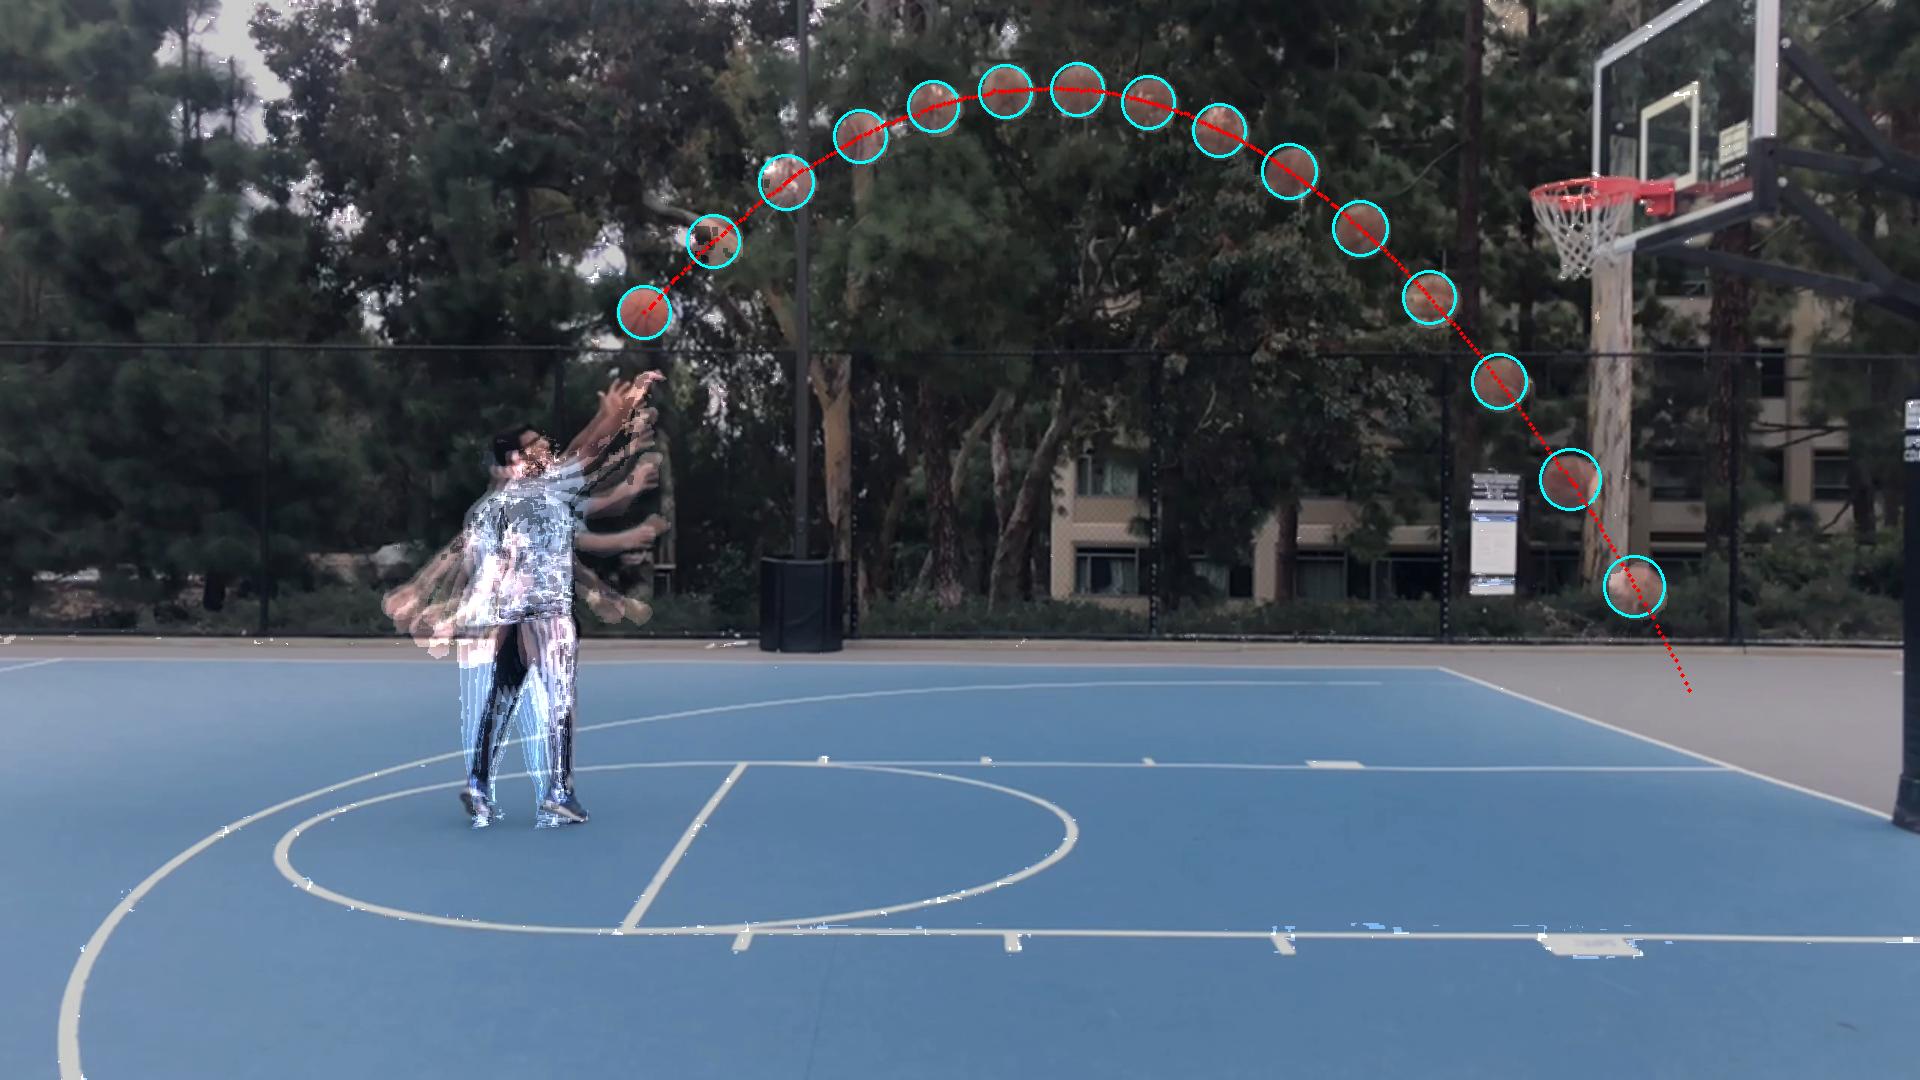
\includegraphics[width=\textwidth]{../results/visualisations/output_Set1_4355-4651.png}
         \caption{Visualisation of ball and bounding circles}
         \label{fig:y equals x}
     \end{subfigure}\\
     \begin{subfigure}[b]{0.7\textwidth}
         \centering
         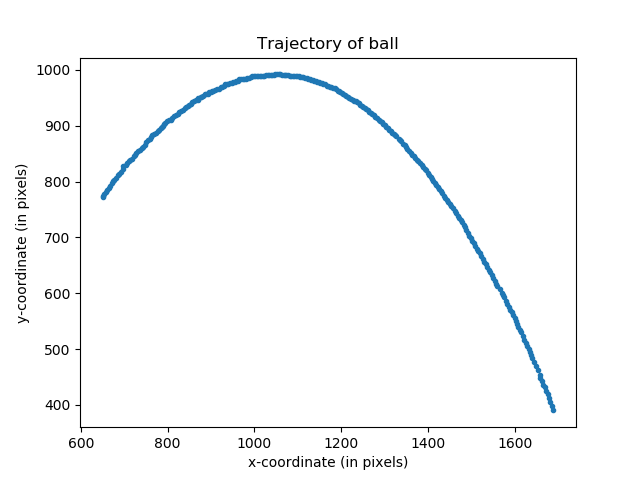
\includegraphics[width=\textwidth]{../results/plots/Set1_4355-4651.png}
         \caption{Plot of the coordinates of the ball detection}
         \label{fig:three sin x}
     \end{subfigure}
     \caption{Results for the video 4355-4651.avi in Set1}
\end{figure}

\begin{figure}[H]
    \centering
    \begin{subfigure}[b]{0.7\textwidth}
         \centering
         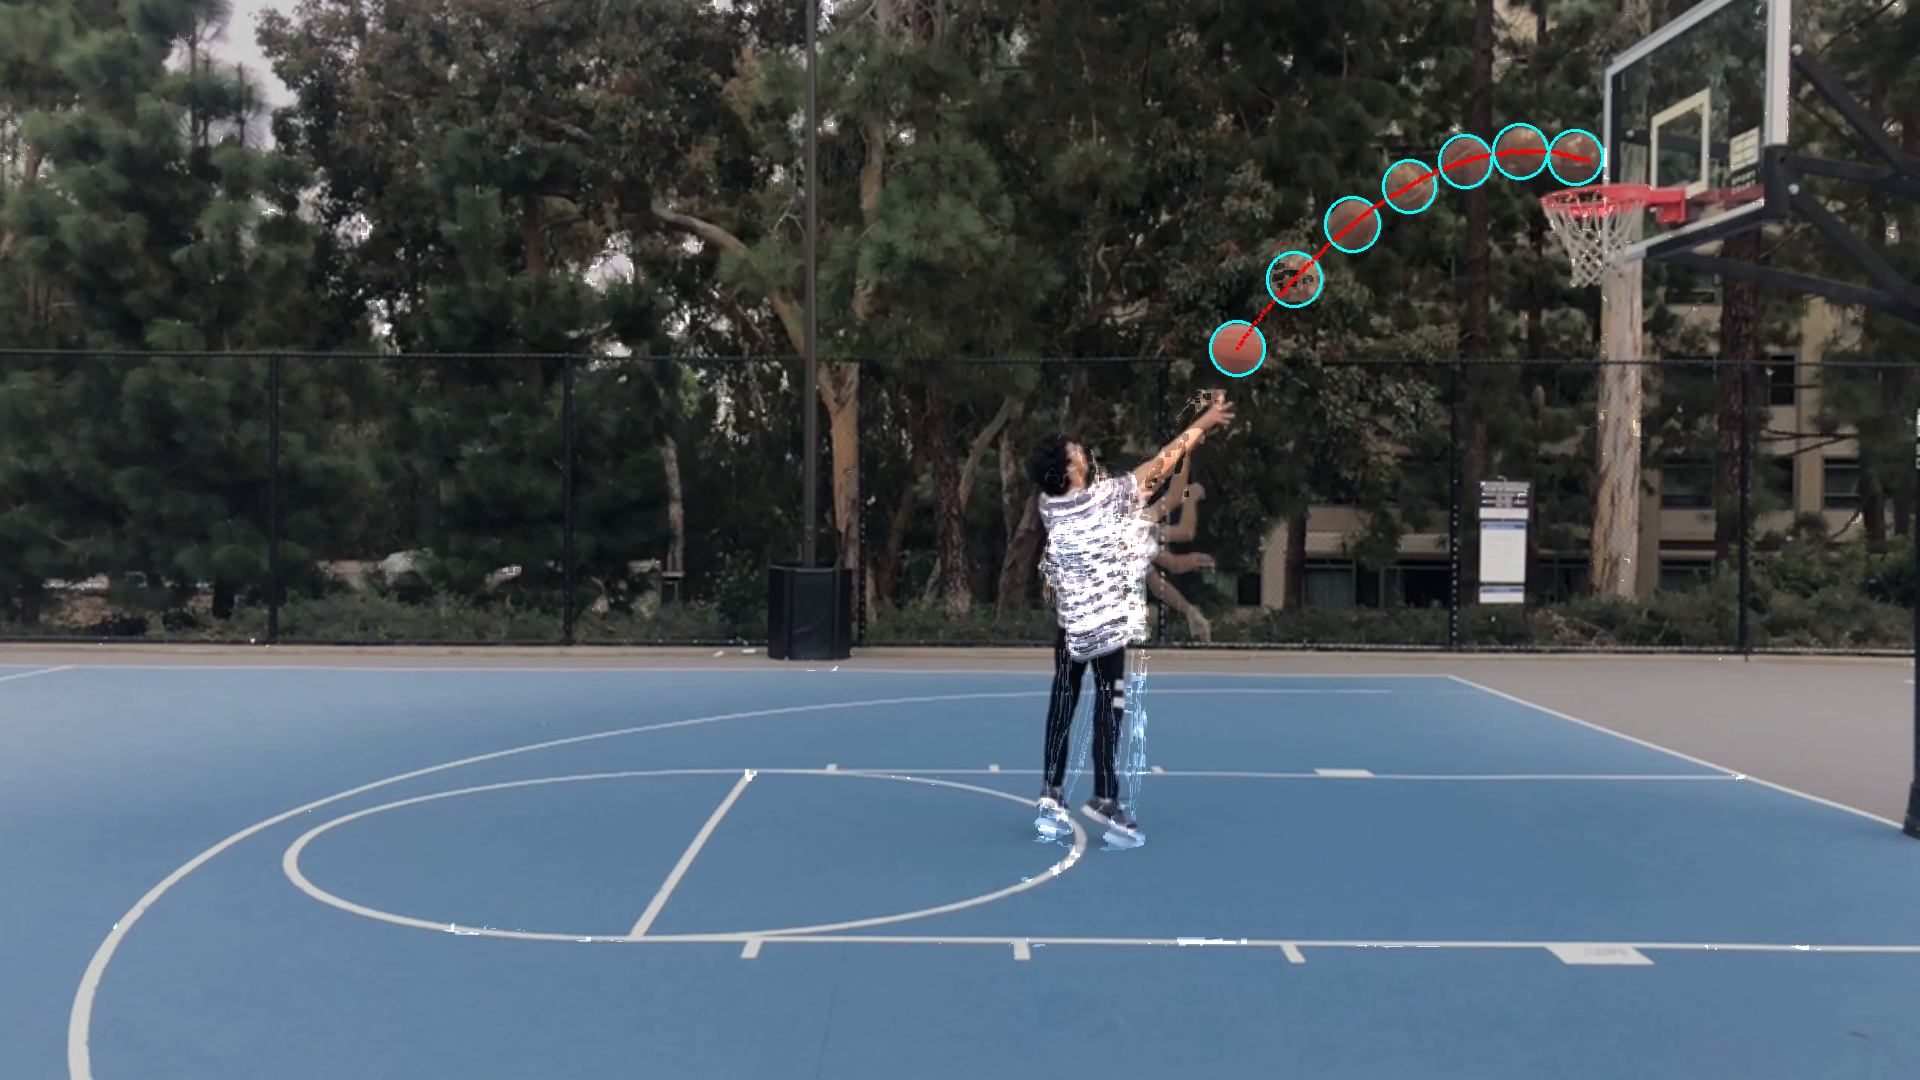
\includegraphics[width=\textwidth]{../results/visualisations/output_Set1_14573-14698.png}
         \caption{Visualisation of ball and bounding circles}
     \end{subfigure}\\
     \begin{subfigure}[b]{0.7\textwidth}
         \centering
         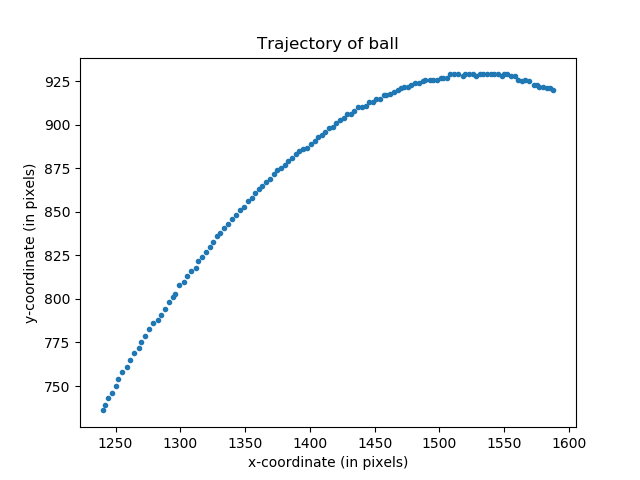
\includegraphics[width=\textwidth]{../results/plots/Set1_14573-14698.png}
         \caption{Plot of the coordinates of the ball detection}
     \end{subfigure}
     \caption{Results for the video 14573-14698.avi in Set1}
\end{figure}

\begin{figure}[H]
    \centering
    \begin{subfigure}[b]{0.7\textwidth}
         \centering
         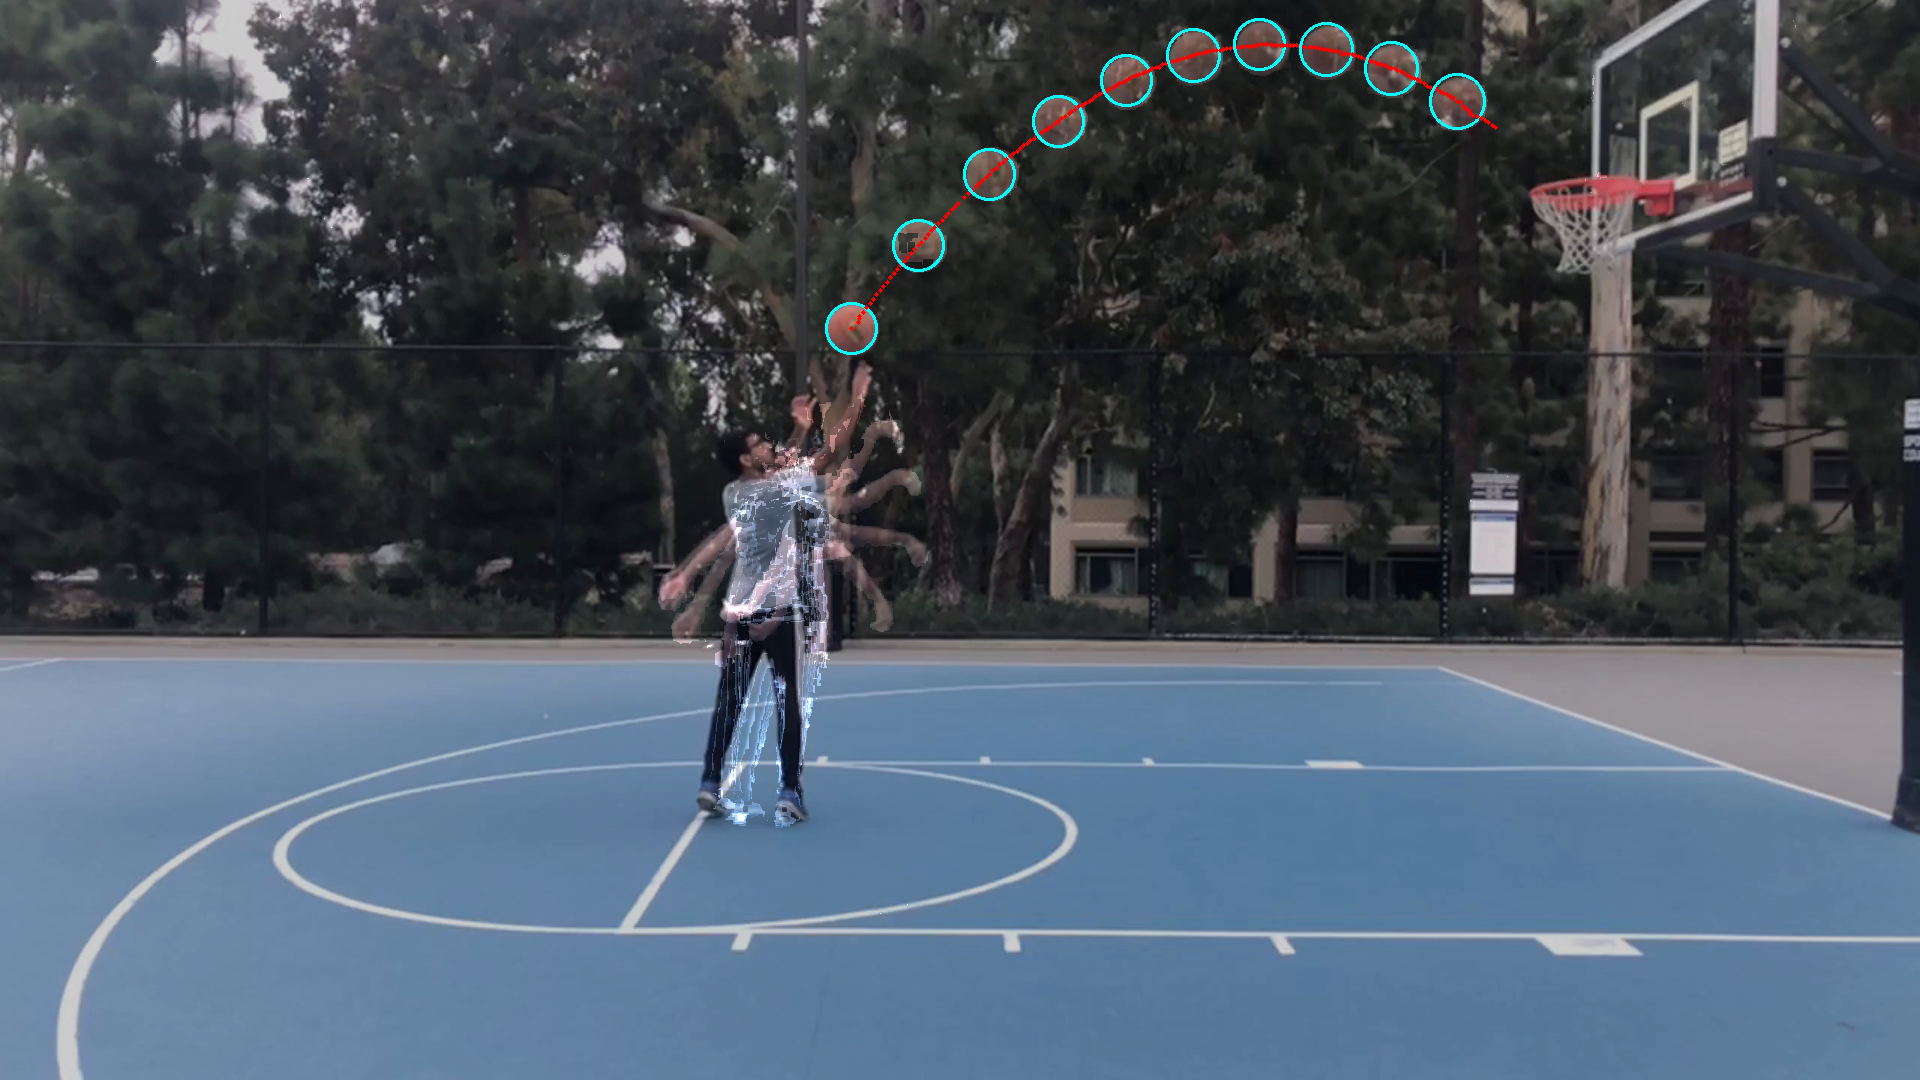
\includegraphics[width=\textwidth]{../results/visualisations/output_Set5_73686-73878.png}
         \caption{Visualisation of ball and bounding circles}
     \end{subfigure}\\
     \begin{subfigure}[b]{0.7\textwidth}
         \centering
         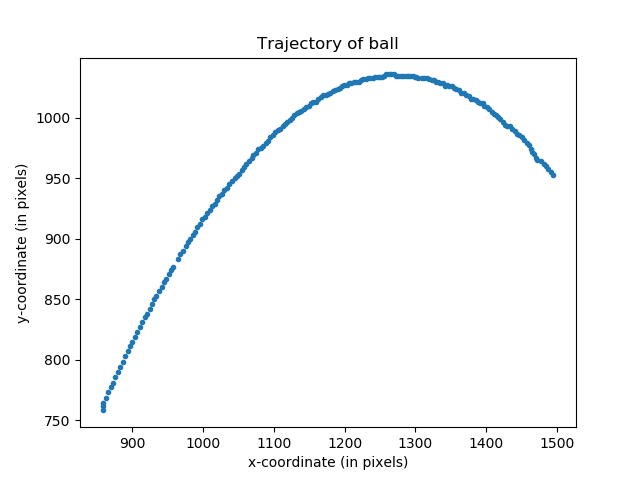
\includegraphics[width=\textwidth]{../results/plots/Set5_73686-73878.png}
         \caption{Plot of the coordinates of the ball detection}
     \end{subfigure}
     \caption{Results for the video 73686-73878.avi in Set5}
\end{figure}

\begin{figure}[H]
    \centering
    \begin{subfigure}[b]{0.7\textwidth}
         \centering
         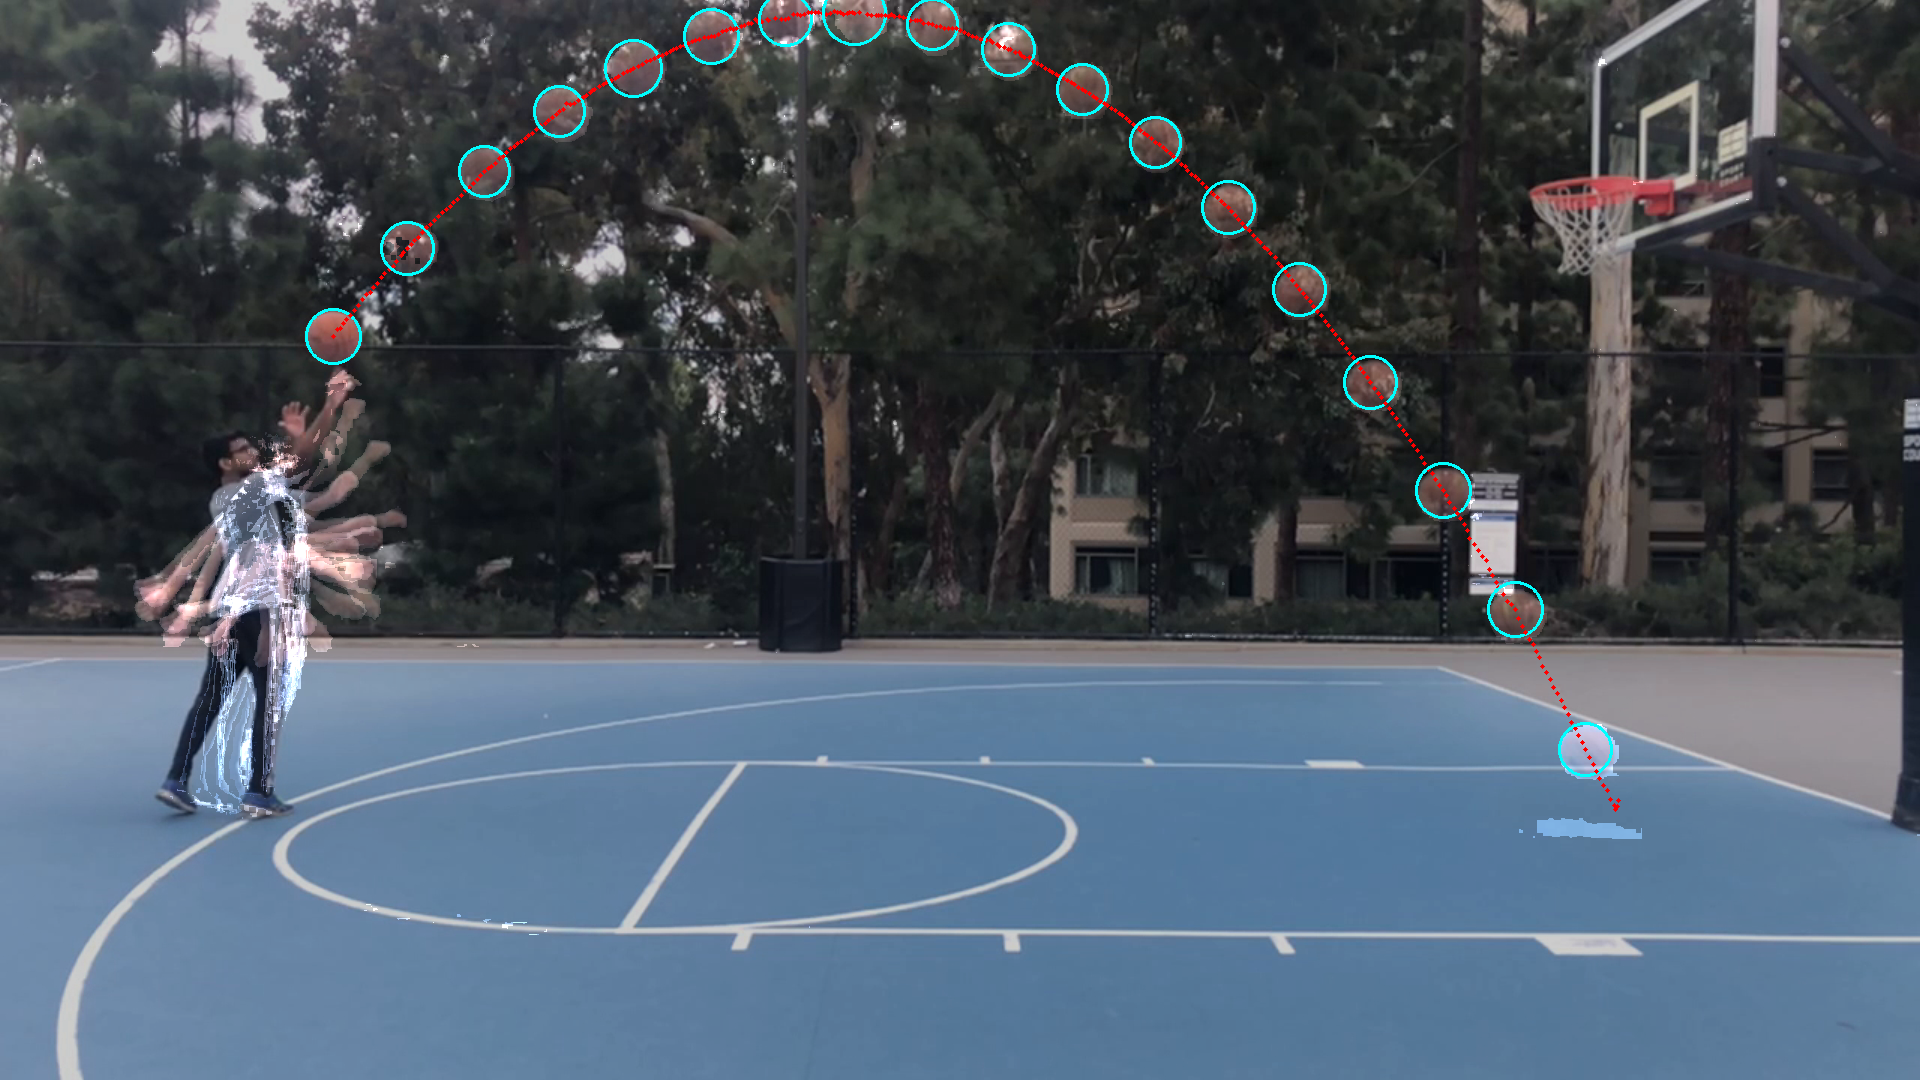
\includegraphics[width=\textwidth]{../results/visualisations/output_Set5_77595-77946.png}
         \caption{Visualisation of ball and bounding circles}
     \end{subfigure}\\
     \begin{subfigure}[b]{0.7\textwidth}
         \centering
         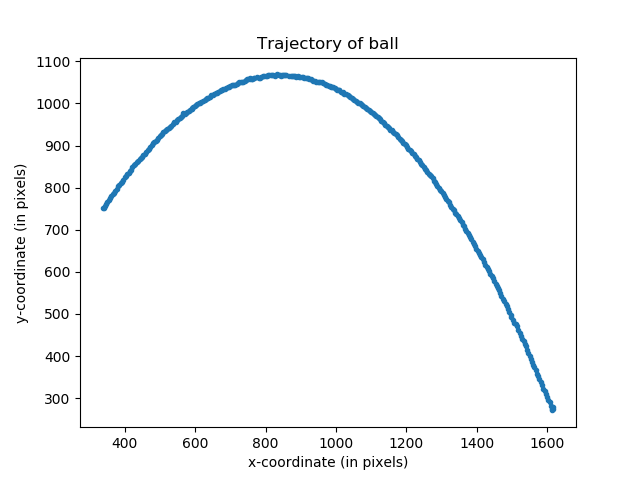
\includegraphics[width=\textwidth]{../results/plots/Set5_77595-77946.png}
         \caption{Plot of the coordinates of the ball detection}
     \end{subfigure}
     \caption{Results for the video 77595-77946.avi in Set5}
\end{figure}

\begin{figure}[H]
    \centering
    \begin{subfigure}[b]{0.7\textwidth}
         \centering
         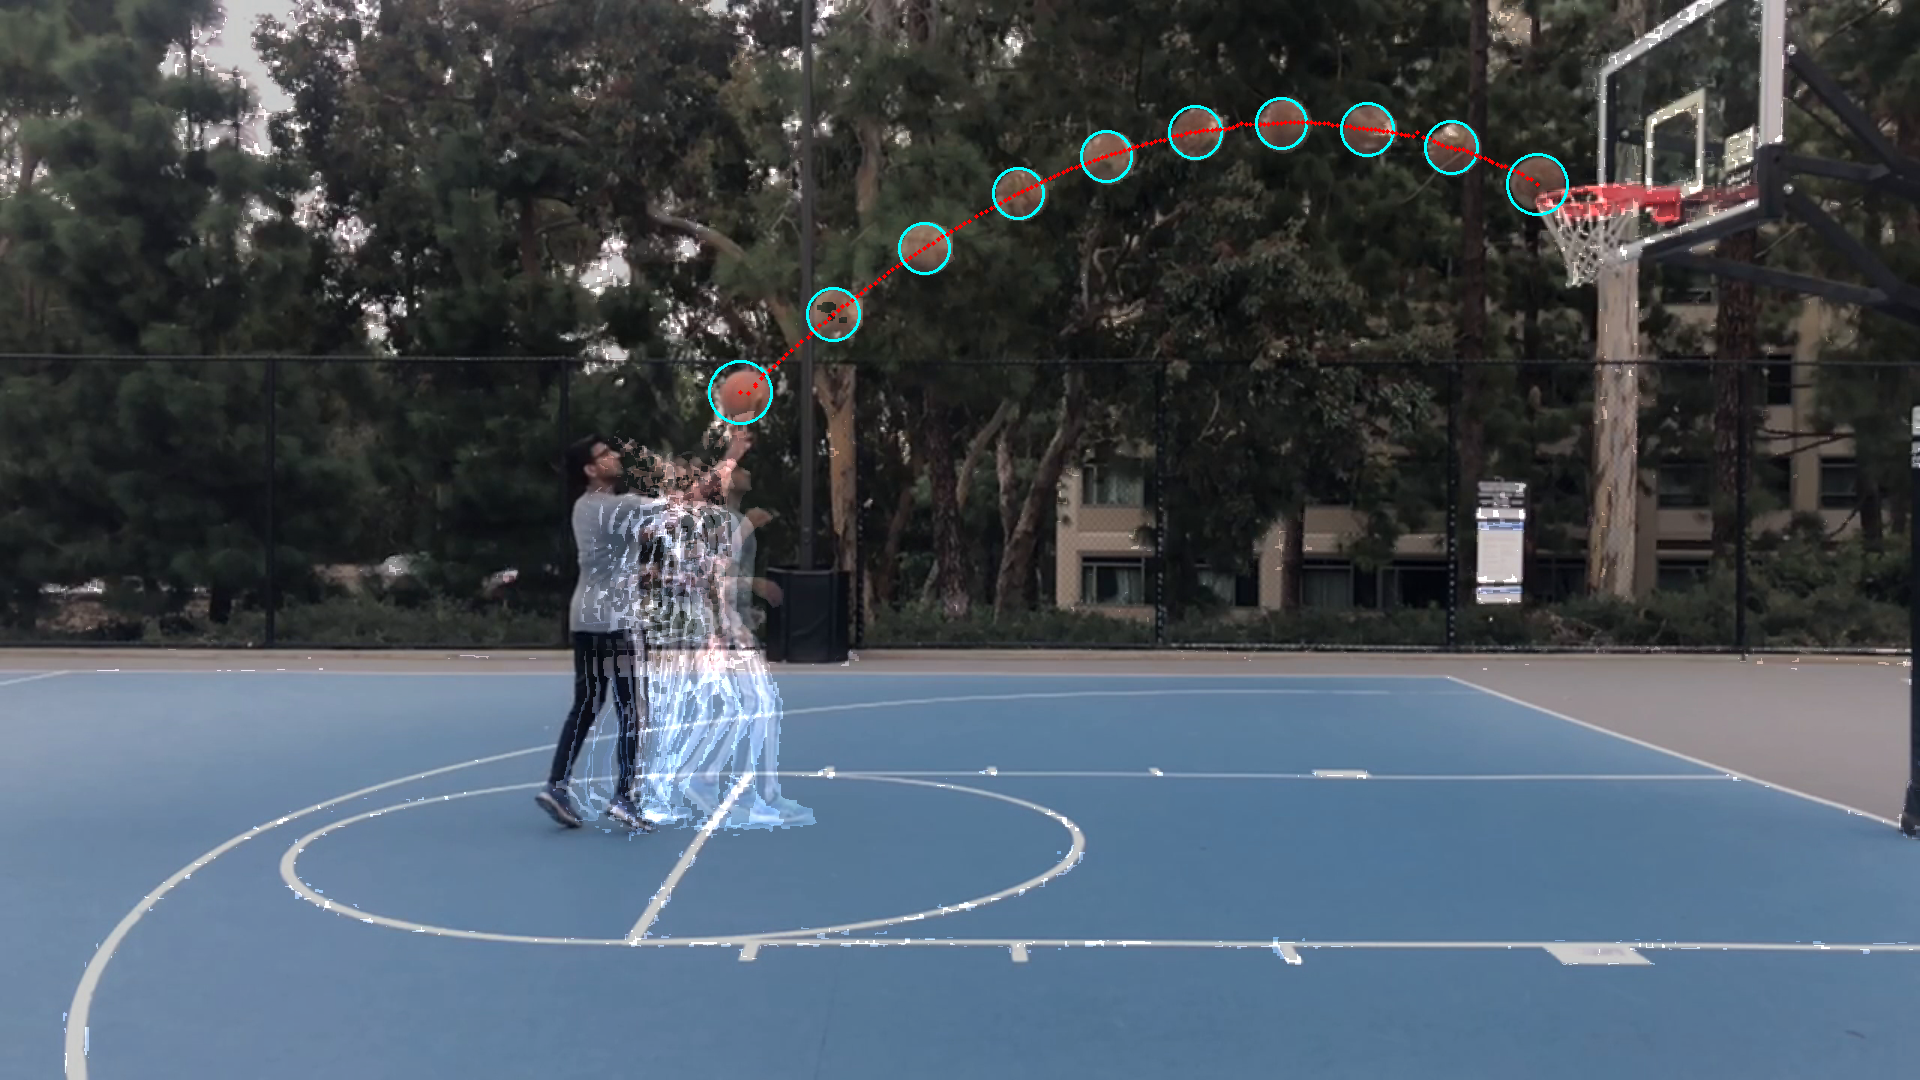
\includegraphics[width=\textwidth]{../results/visualisations/output_Set23_94026-94206.png}
         \caption{Visualisation of ball and bounding circles}
     \end{subfigure}\\
     \begin{subfigure}[b]{0.7\textwidth}
         \centering
         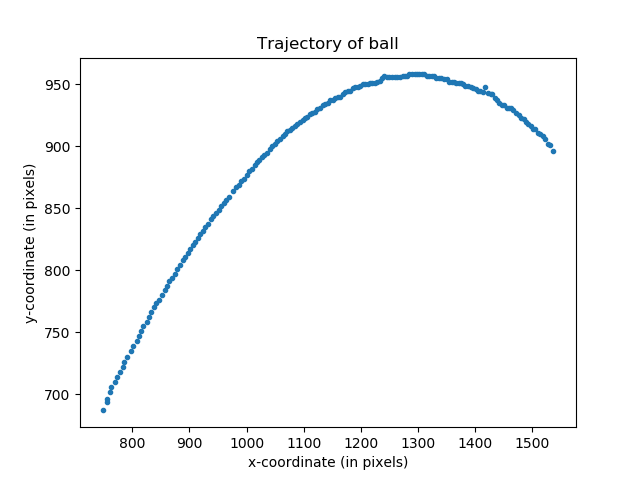
\includegraphics[width=\textwidth]{../results/plots/Set23_94026-94206.png}
         \caption{Plot of the coordinates of the ball detection}
     \end{subfigure}
     \caption{Results for the video 94026-94206.avi in Set23}
\end{figure}

The case below shows that these assumptions can give noisy results in some situations. However, it was observed that the assumptions and the tuned parameters worked reasonably well for most videos.

\begin{figure}[H]
    \centering
    \begin{subfigure}[b]{0.7\textwidth}
         \centering
         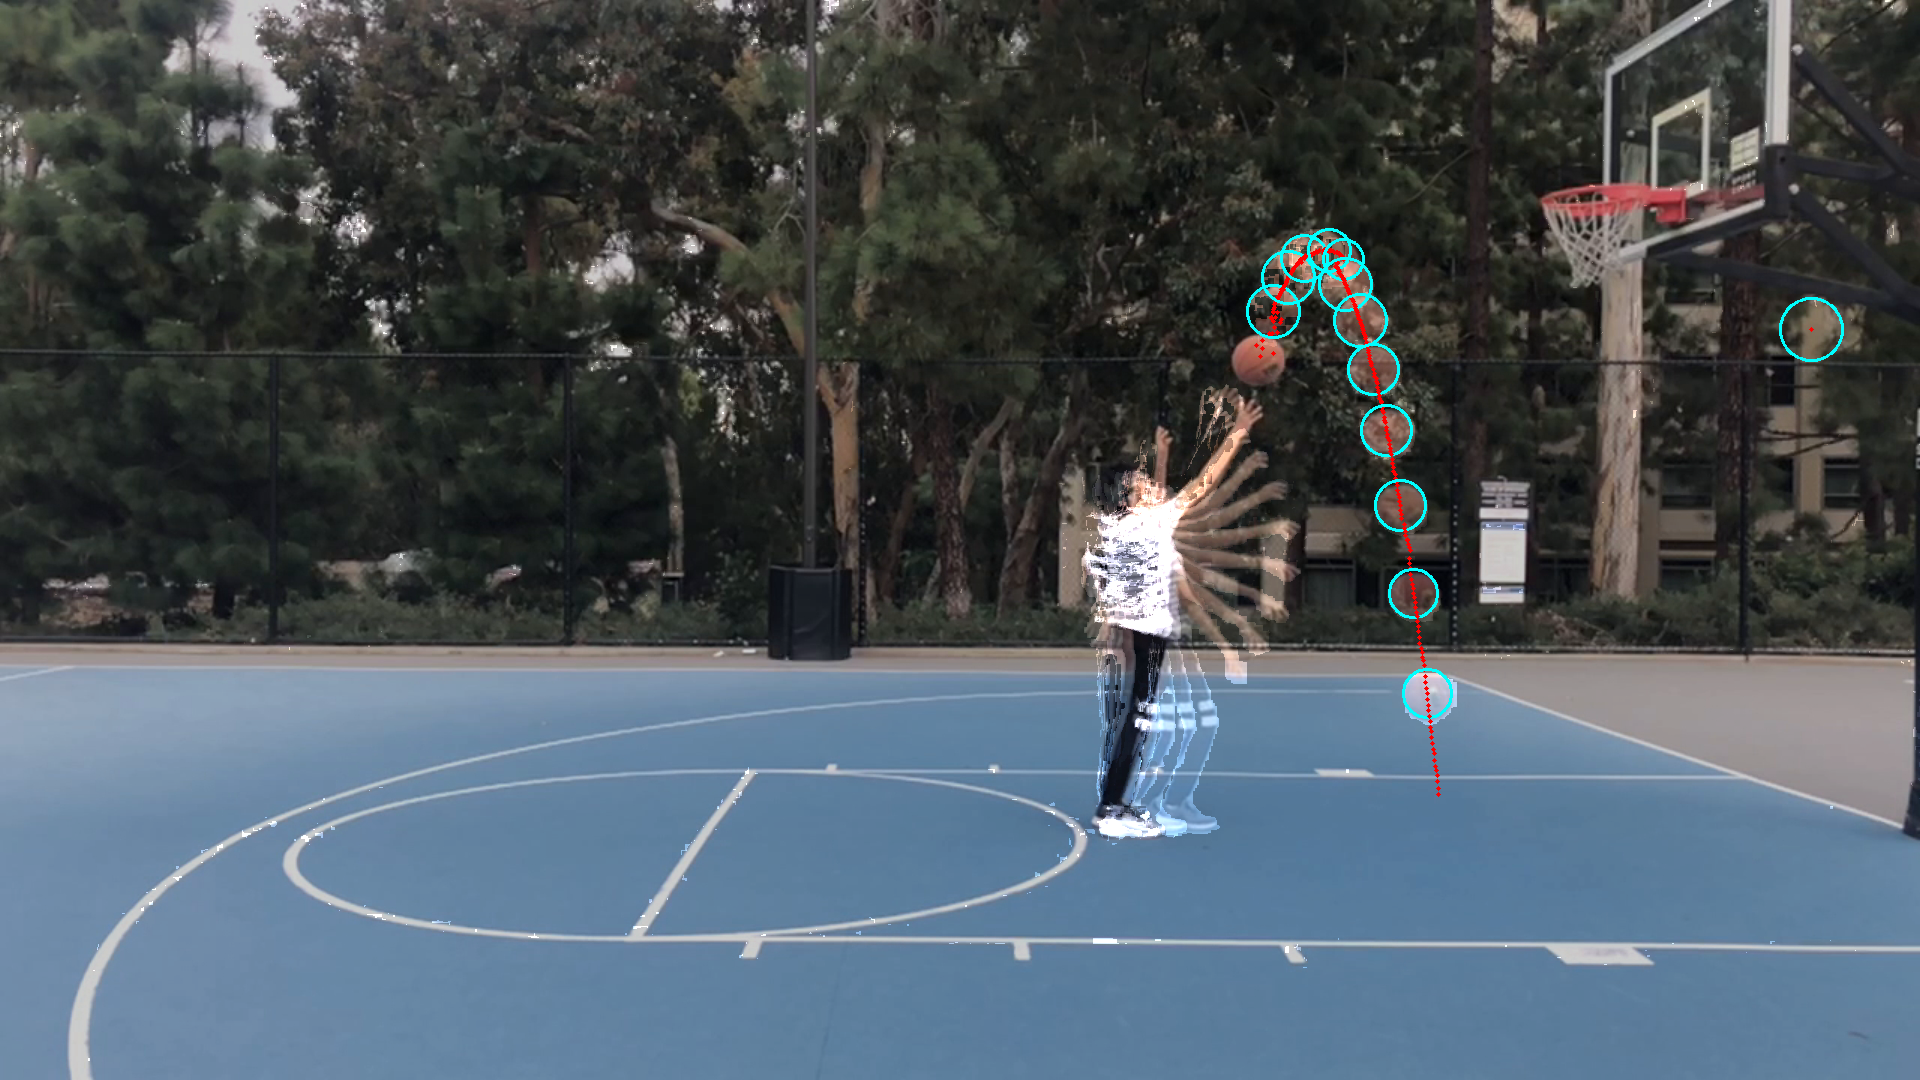
\includegraphics[width=\textwidth]{../results/visualisations/output_Set1_6720-6978.png}
         \caption{Visualisation of ball and bounding circles}
     \end{subfigure}\\
     \begin{subfigure}[b]{0.7\textwidth}
         \centering
         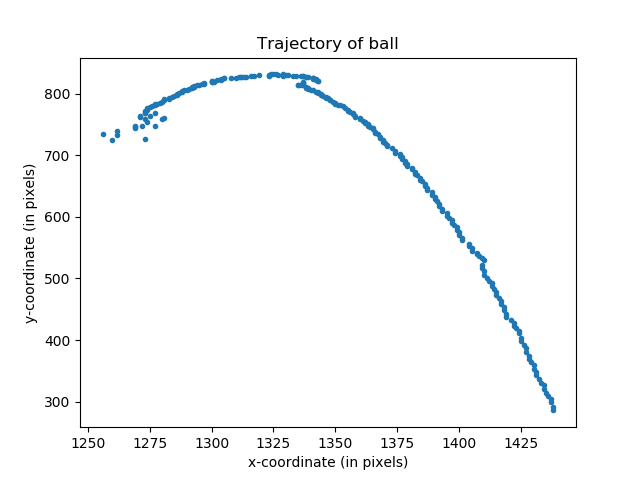
\includegraphics[width=\textwidth]{../results/plots/Set1_6720-6978.png}
         \caption{Plot of the coordinates of the ball detection}
     \end{subfigure}
     \caption{Results for the video 6720-6978.avi in Set1}
\end{figure}


\section*{Conclusion}
A method for object detection using traditional computer vision techniques is demonstrated. Under certain assumption on the dataset, it is shown qualitatively that this approach work reasonably well for most of the videos in the dataset. Excluding the time taken to read each frame and displaying it, the time taken for the complete detection operation is around 0.04 seconds per frame, which is about 25 fps on a Dual-Core Inter i5 processor.
\end{document}
